% This is "sig-alternate.tex" V1.8 June 2007 Modified for SOUPS 2014
% This file should be compiled with V2.3 of "sig-alternate.cls" June 2007
%
% This example file demonstrates the use of the 'sig-alternate.cls'
% V2.3 LaTeX2e document class file. It is for those submitting
% articles to ACM Conference Proceedings WHO DO NOT WISH TO
% STRICTLY ADHERE TO THE SIGS (PUBS-BOARD-ENDORSED) STYLE.
% The 'sig-alternate.cls' file will produce a similar-looking,
% albeit, 'tighter' paper resulting in, invariably, fewer pages.
%
% ----------------------------------------------------------------------------------------------------------------
% This .tex file (and associated .cls V2.3) produces:
%       1) The Permission Statement
%       2) The Conference (location) Info information
%       3) The Copyright Line with ACM data
%       4) NO page numbers
%
% as against the acm_proc_article-sp.cls file which
% DOES NOT produce 1) thru' 3) above.
%
% Using 'sig-alternate.cls' you have control, however, from within
% the source .tex file, over both the CopyrightYear
% (defaulted to 200X) and the ACM Copyright Data
% (defaulted to X-XXXXX-XX-X/XX/XX).
% e.g.
% \CopyrightYear{2007} will cause 2007 to appear in the copyright line.
% \crdata{0-12345-67-8/90/12} will cause 0-12345-67-8/90/12 to appear in the copyright line.
%
% ---------------------------------------------------------------------------------------------------------------
% This .tex source is an example which *does* use
% the .bib file (from which the .bbl file % is produced).
% REMEMBER HOWEVER: After having produced the .bbl file,
% and prior to final submission, you *NEED* to 'insert'
% your .bbl file into your source .tex file so as to provide
% ONE 'self-contained' source file.
%
% ================= IF YOU HAVE QUESTIONS =======================
% Questions regarding the SIGS styles, SIGS policies and
% procedures, Conferences etc. should be sent to
% Adrienne Griscti (griscti@acm.org)
%
% Technical questions _only_ to
% Gerald Murray (murray@acm.org)
% ===============================================================
%
% For tracking purposes - this is V1.8 - June 2007

% --- Start page size ---
%Please use the following format  
\documentclass[twoside,letterpaper]{soups} 
\pdfpagewidth=8.5truein 
\pdfpageheight=11truein 
% --- End page size ---


\usepackage{graphicx}
\usepackage{times}
\renewcommand{\topfraction}{0.99} % be more aggressive about text around floats
\renewcommand{\floatpagefraction}{0.99}
\pagestyle{plain} % page numbers

\begin{document}
%
% --- Author Metadata here ---
\conferenceinfo{Symposium on Usable Privacy and Security
  (SOUPS)}{2016, June 22--24, 2016, Denver, Colorado.}
\CopyrightYear{2016} % Allows default copyright year (200X) to be over-ridden - IF NEED BE.
%\crdata{0-12345-67-8/90/01}  % Allows default copyright data (0-89791-88-6/97/05) to be over-ridden - IF NEED BE.
% --- End of Author Metadata ---

\title{Our Workshop Paper in the SOUPS 2016 Template. Please look at the aside, methodology, and results%
\titlenote{(Produces the permission block, and copyright information). For use with SIG-ALTERNATE.CLS. Supported by ACM.}}
\subtitle{Subtitle (optional)%
\titlenote{A full version of this paper is available as
\textit{Author's Guide to Preparing ACM SIG Proceedings Using
\LaTeX$2_\epsilon$\ and BibTeX} at
\texttt{www.acm.org/sigs/publications/sigguide-v2.2sp}}}
%
% You need the command \numberofauthors to handle the 'placement
% and alignment' of the authors beneath the title.
%
% For aesthetic reasons, we recommend 'three authors at a time'
% i.e. three 'name/affiliation blocks' be placed beneath the title.
%
% NOTE: You are NOT restricted in how many 'rows' of
% "name/affiliations" may appear. We just ask that you restrict
% the number of 'columns' to three.
%
% Because of the available 'opening page real-estate'
% we ask you to refrain from putting more than six authors
% (two rows with three columns) beneath the article title.
% More than six makes the first-page appear very cluttered indeed.
%
% Use the \alignauthor commands to handle the names
% and affiliations for an 'aesthetic maximum' of six authors.
% Add names, affiliations, addresses for
% the seventh etc. author(s) as the argument for the
% \additionalauthors command.
% These 'additional authors' will be output/set for you
% without further effort on your part as the last section in
% the body of your article BEFORE References or any Appendices.

\numberofauthors{8} %  in this sample file, there are a *total*
% of EIGHT authors. SIX appear on the 'first-page' (for formatting
% reasons) and the remaining two appear in the \additionalauthors section.
%
\author{
% You can go ahead and credit any number of authors here,
% e.g. one 'row of three' or two rows (consisting of one row of three
% and a second row of one, two or three).
%
% The command \alignauthor (no curly braces needed) should
% precede each author name, affiliation/snail-mail address and
% e-mail address. Additionally, tag each line of
% affiliation/address with \affaddr, and tag the
% e-mail address with \email.
%
% 1st. author
\alignauthor
Tyler W Thomas\titlenote{author 1 note here.}\\
       \affaddr{Institute for Clarity in Documentation}\\
       \affaddr{1932 Wallamaloo Lane}\\
       \affaddr{Wallamaloo, New Zealand}\\
       \email{trovato@corporation.com}
% 2nd. author
\alignauthor
Justin Smith\titlenote{author 2 note here}\\
       \affaddr{Institute for Clarity in Documentation}\\
       \affaddr{P.O. Box 1212}\\
       \affaddr{Dublin, Ohio 43017-6221}\\
       \email{webmaster@marysville-ohio.com}
% 3rd. author
\alignauthor Heather Lipford{\o}rv{\"a}ld\titlenote{author 3 note here}\\
       \affaddr{The Th{\o}rv{\"a}ld Group}\\
       \affaddr{1 Th{\o}rv{\"a}ld Circle}\\
       \affaddr{Hekla, Iceland}\\
       \email{larst@affiliation.org}
\and  % use '\and' if you need 'another row' of author names
% 4th. author
\alignauthor Bill Chu\\
       \affaddr{Brookhaven Laboratories}\\
       \affaddr{Brookhaven National Lab}\\
       \affaddr{P.O. Box 5000}\\
       \email{lleipuner@researchlabs.org}
% 5th. author
\alignauthor Emerson Murphy-Hill\\
       \affaddr{NASA Ames Research Center}\\
       \affaddr{Moffett Field}\\
       \affaddr{California 94035}\\
       \email{fogartys@amesres.org}
}
% There's nothing stopping you putting the seventh, eighth, etc.
% author on the opening page (as the 'third row') but we ask,
% for aesthetic reasons that you place these 'additional authors'
% in the \additional authors block, viz.
\additionalauthors{Additional authors: John Smith (The Th{\o}rv{\"a}ld Group,
email: {\texttt{jsmith@affiliation.org}}) and Julius P.~Kumquat
(The Kumquat Consortium, email: {\texttt{jpkumquat@consortium.net}}).}
\date{30 July 1999}
% Just remember to make sure that the TOTAL number of authors
% is the number that will appear on the first page PLUS the
% number that will appear in the \additionalauthors section.

\maketitle
\begin{abstract}
This paper provides a sample of a \LaTeX\ document which conforms,
somewhat loosely, to the formatting guidelines for
ACM SIG Proceedings. It is an {\em alternate} style which produces
a {\em tighter-looking} paper and was designed in response to
concerns expressed, by authors, over page-budgets.
It complements the document \textit{Author's (Alternate) Guide to
Preparing ACM SIG Proceedings Using \LaTeX$2_\epsilon$\ and Bib\TeX}.
This source file has been written with the intention of being
compiled under \LaTeX$2_\epsilon$\ and BibTeX.

The developers have tried to include every imaginable sort
of ``bells and whistles," such as a subtitle, footnotes on
title, subtitle and authors, as well as in the text, and
every optional component (e.g. Acknowledgments, Additional
Authors, Appendices), not to mention examples of
equations, theorems, tables and figures.

To make best use of this sample document, run it through \LaTeX\
and BibTeX, and compare this source code with the printed
output produced by the dvi file. A compiled PDF version
is available on the web page to help you with the
`look and feel'.
\end{abstract}


\section{Introduction}
The \textit{proceedings} are the records of a conference.
SOUPS hopes to give these conference by-products a uniform,
high-quality appearance.  To do this, there are some rigid
requirements for the format of the proceedings documents: there
is a specified format (balanced  double columns), a specified
set of fonts (Arial or Helvetica and Times Roman) in
certain specified sizes (for instance, 9 point for body copy),
a specified live area (18 $\times$ 23.5 cm [7" $\times$ 9.25"]) centered on
the page, specified size of margins (2.54cm [1"] top and
bottom and 1.9cm [.75"] left and right; specified column width
(8.45cm [3.33"]) and gutter size (.083cm [.33"]).

The good news is, with only a handful of manual
settings\footnote{Two of these, the {\texttt{\char'134 numberofauthors}}
and {\texttt{\char'134 alignauthor}} commands, you have
already used; another, {\texttt{\char'134 balancecolumns}}, will
be used in your very last run of \LaTeX\ to ensure
balanced column heights on the last page.}, the \LaTeX\ document
class file handles all of this for you.

The remainder of this document is concerned with showing, in
the context of an ``actual'' document, the \LaTeX\ commands
specifically available for denoting the structure of a
proceedings paper, rather than with giving rigorous descriptions
or explanations of such commands.

\section{The {\secit Body} of The Paper}
Typically, the body of a paper is organized
into a hierarchical structure, with numbered or unnumbered
headings for sections, subsections, sub-subsections, and so on. 
The command \texttt{{\char'134}section} that
precedes this paragraph is part of such a
hierarchy.\footnote{This is the second footnote.  It
starts a series of three footnotes that add nothing
informational, but just give an idea of how footnotes work
and look. It is a wordy one, just so you see
how a longish one plays out.} \LaTeX\ handles the numbering
and placement of these headings for you, when you use
the appropriate heading commands around the titles
of the headings.  If you want a sub-subsection or
smaller part to be unnumbered in your output, simply append an
asterisk to the command name.  Examples of both
numbered and unnumbered headings will appear throughout the
balance of this sample document.

Because the entire article is contained in
the \textbf{document} environment, you can indicate the
start of a new paragraph with a blank line in your
input file; that is why this sentence forms a separate paragraph.

\subsection{Type Changes and {\subsecit Special} Characters}
We have already seen several typeface changes in this sample.  You
can indicate italicized words or phrases in your text with
the command \texttt{{\char'134}textit}; emboldening with the
command \texttt{{\char'134}textbf}
and typewriter-style (for instance, for computer code) with
\texttt{{\char'134}texttt}.  But remember, you do not
have to indicate typestyle changes when such changes are
part of the \textit{structural} elements of your
article; for instance, the heading of this subsection will
be in a sans serif\footnote{A third footnote, here.
Let's make this a rather short one to
see how it looks.} typeface, but that is handled by the
document class file. Take care with the use
of\footnote{A fourth, and last, footnote.}
the curly braces in typeface changes; they mark
the beginning and end of
the text that is to be in the different typeface.

You can use whatever symbols, accented characters, or
non-English characters you need anywhere in your document;
you can find a complete list of what is
available in the \textit{\LaTeX\
User's Guide} \cite{Lamport:LaTeX}.

\subsection{Math Equations}
You may want to display math equations in three distinct styles:
inline, numbered, or non-numbered display.  Each of
the three are discussed in the next sections.

\subsubsection{Inline (In-text) Equations}
A formula that appears in the running text is called an
inline or in-text formula.  It is produced by the
\textbf{math} environment, which can be
invoked with the usual \texttt{{\char'134}begin. . .{\char'134}end}
construction or with the short form \texttt{\$. . .\$}. You
can use any of the symbols and structures,
from $\alpha$ to $\omega$, available in
\LaTeX\cite{Lamport:LaTeX}; this section will simply show a
few examples of in-text equations in context. Notice how
this equation: \begin{math}\lim_{n\rightarrow \infty}x=0\end{math},
set here in in-line math style, looks slightly different when
set in display style.  (See next section).

\subsubsection{Display Equations}
A numbered display equation -- one set off by vertical space
from the text and centered horizontally -- is produced
by the \textbf{equation} environment. An unnumbered display
equation is produced by the \textbf{displaymath} environment.

Again, in either environment, you can use any of the symbols
and structures available in \LaTeX; this section will just
give a couple of examples of display equations in context.
First, consider the equation, shown as an inline equation above:
\begin{equation}\lim_{n\rightarrow \infty}x=0\end{equation}
Notice how it is formatted somewhat differently in
the \textbf{displaymath}
environment.  Now, we'll enter an unnumbered equation:
\begin{displaymath}\sum_{i=0}^{\infty} x + 1\end{displaymath}
and follow it with another numbered equation:
\begin{equation}\sum_{i=0}^{\infty}x_i=\int_{0}^{\pi+2} f\end{equation}
just to demonstrate \LaTeX's able handling of numbering.

\subsection{Citations}
Citations to articles \cite{bowman:reasoning,
braams:babel, clark:pct, herlihy:methodology},
conference proceedings \cite{clark:pct} or
books \cite{Lamport:LaTeX, salas:calculus} listed
in the Bibliography (or ``References'') section of your
article will occur throughout the text of your article.
You should use BibTeX to automatically produce this bibliography;
you simply need to insert one of several citation commands with
a key of the item cited in the proper location in
the \texttt{.tex} file \cite{Lamport:LaTeX}.
The key is a short reference you invent to uniquely
identify each work; in this sample document, the key is
the first author's surname and a
word from the title.  This identifying key is included
with each item in the \texttt{.bib} file for your article.

The details of the construction of the \texttt{.bib} file
are beyond the scope of this sample document, but more
information can be found in the \textit{Author's Guide},
and exhaustive details in the \textit{\LaTeX\ User's
Guide}\cite{Lamport:LaTeX}.

This article shows only the plainest form
of the citation command, using \texttt{{\char'134}cite}.
This is what is stipulated in the SIGS style specifications.
No other citation format is endorsed or supported.

Your reference list should be ordered alphabetically. When
citing more than one reference in the same set of brackets,
list the papers in ascending numerical order e.g., [1,2,3].

\subsection{Tables}
Because tables cannot be split across pages, the best
placement for them is typically the top of the page
nearest their initial cite.  To
ensure this proper ``floating'' placement of tables, use the
environment \textbf{table} to enclose the table's contents and
the table caption.  The contents of the table itself must go
in the \textbf{tabular} environment, to
be aligned properly in rows and columns, with the desired
horizontal and vertical rules.  Again, detailed instructions
on \textbf{tabular} material
is found in the \textit{\LaTeX\ User's Guide}.

Immediately following this sentence is the point at which
Table 1 is included in the input file; compare the
placement of the table here with the table in the printed
dvi output of this document.

\begin{table}
\centering
\caption{Frequency of Special Characters.}
\begin{tabular}{|c|c|l|} \hline
Non-English or Math&Frequency&Comments\\ \hline
\O & 1 in 1,000& For Swedish names\\ \hline
$\pi$ & 1 in 5& Common in math\\ \hline
\$ & 4 in 5 & Used in business\\ \hline
$\Psi^2_1$ & 1 in 40,000& Unexplained usage\\
\hline\end{tabular}
\end{table}

To set a wider table, which takes up the whole width of
the page's live area, use the environment
\textbf{table*} to enclose the table's contents and
the table caption.  As with a single-column table, this wide
table will ``float" to a location deemed more desirable.
Immediately following this sentence is the point at which
Table 2 is included in the input file; again, it is
instructive to compare the placement of the
table here with the table in the printed dvi
output of this document.


\begin{table*}
\centering
\caption{Some Typical Commands}
\begin{tabular}{|c|c|l|} \hline
Command&A Number&Comments\\ \hline
\texttt{{\char'134}alignauthor} & 100& Author alignment\\ \hline
\texttt{{\char'134}numberofauthors}& 200& Author enumeration\\ \hline
\texttt{{\char'134}table}& 300 & For tables\\ \hline
\texttt{{\char'134}table*}& 400& For wider tables\\ \hline\end{tabular}
\end{table*}
% end the environment with {table*}, NOTE not {table}!

\subsection{Figures}
Like tables, figures cannot be split across pages; the
best placement for them
is typically the top or the bottom of the page nearest
their initial cite.  To ensure this proper ``floating'' placement
of figures, use the environment
\textbf{figure} to enclose the figure and its caption.

This sample document contains examples of \textbf{.pdf}
files to be displayable with \LaTeX.  More
details on each of these is found in the \textit{Author's Guide}.

\begin{figure}
\centering

\includegraphics{fly}
\caption{A sample black and white graphic (.pdf format).}
\end{figure}

\begin{figure}
\centering

\includegraphics[height=1in,width=1in]{fly}
\caption{A sample black and white graphic (.pdf format)
that has been resized with the \texttt{includegraphics} command.}
\end{figure}


As was the case with tables, you may want a figure
that spans two columns.  To do this, and still to
ensure proper ``floating'' placement of tables, use the environment
\textbf{figure*} to enclose the figure and its caption.
\begin{figure*}
\centering
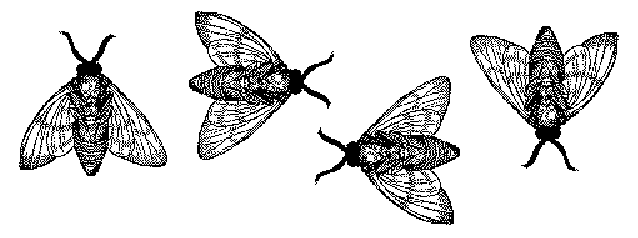
\includegraphics{flies}
\caption{A sample black and white graphic (.pdf format)
that spans two columns of text.}
\end{figure*}
and don't forget to end the environment with
{figure*}, not {figure}!

Note that either {\textbf{.pdf}} or {\textbf{.jpeg}} formats can be
included with the \verb+\includegraphics+ command.

\begin{figure}
\centering
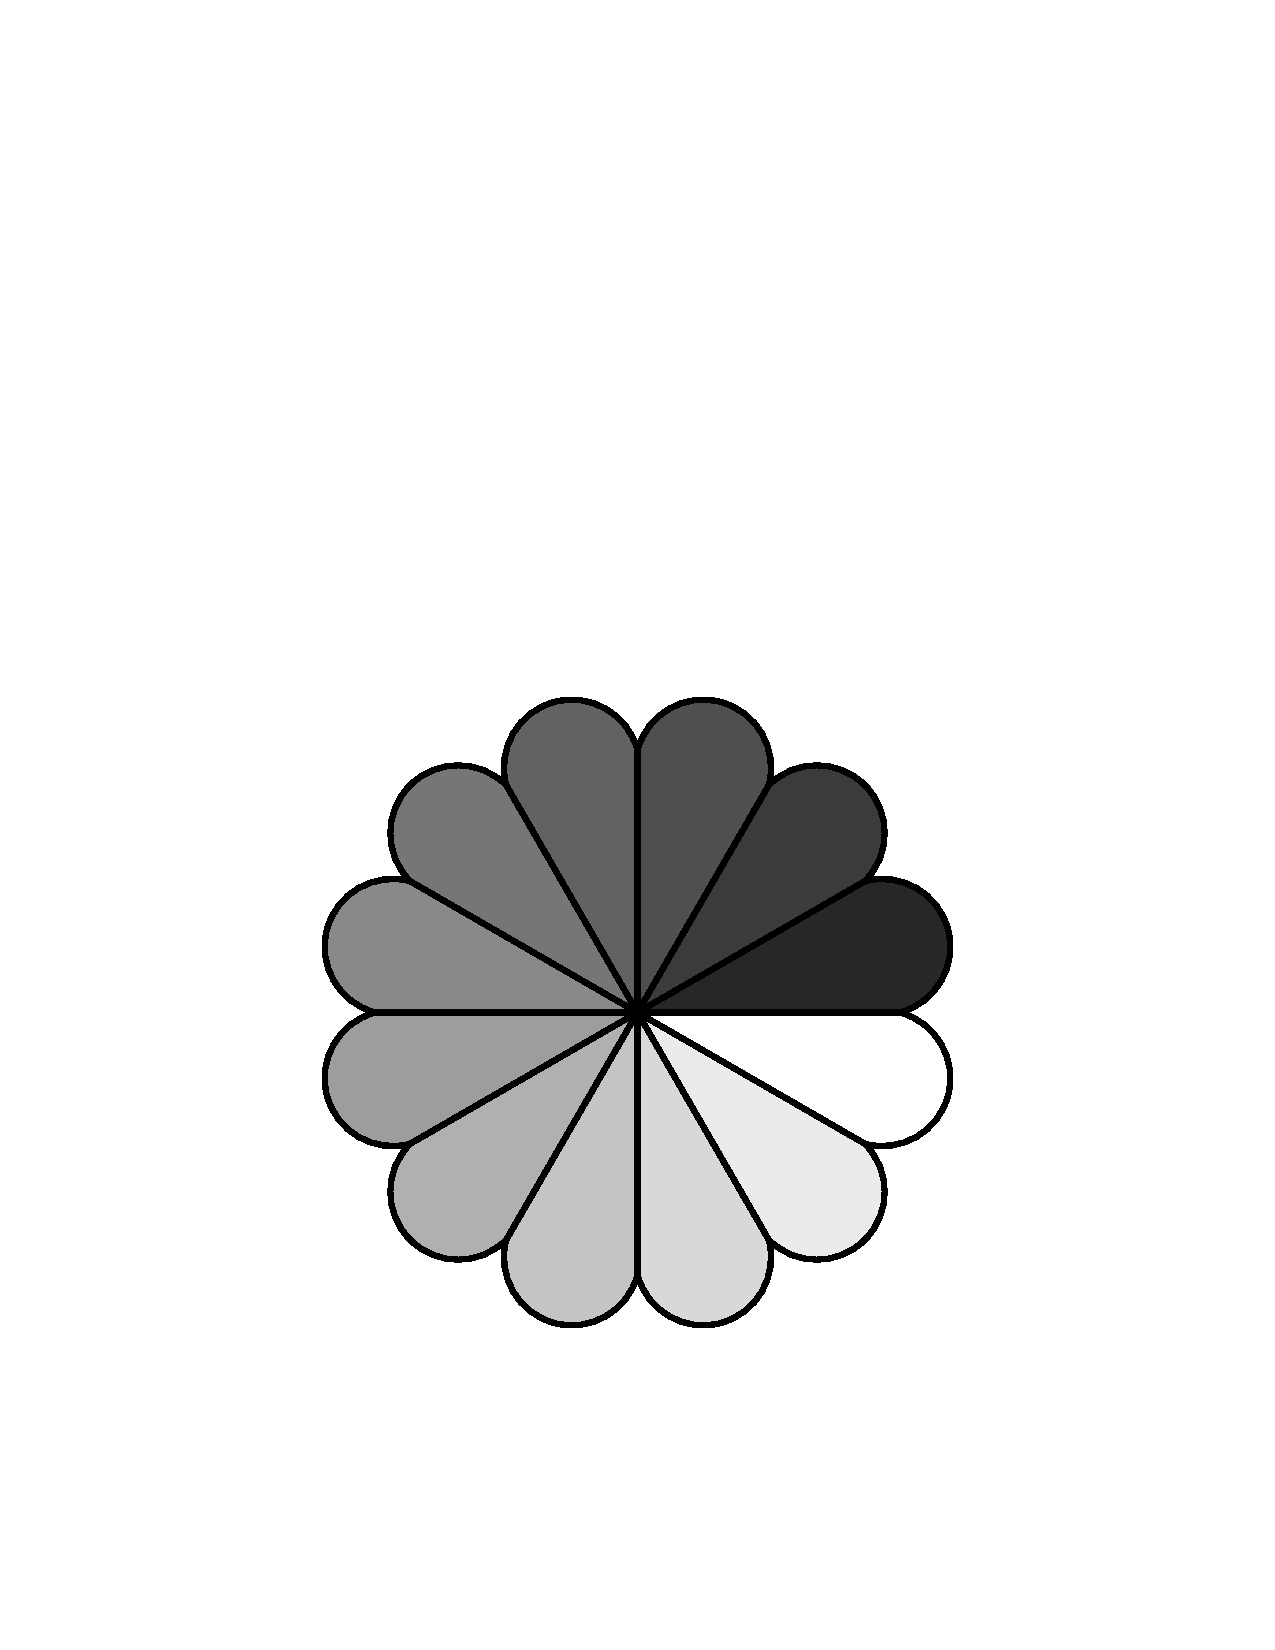
\includegraphics[height=1in,width=1in]{rosette}
\caption{A sample black and white graphic (.pdf format) that has
been resized with the \texttt{includegraphics} command.}
\vskip -6pt
\end{figure}

\subsection{Theorem-like Constructs}
Other common constructs that may occur in your article are
the forms for logical constructs like theorems, axioms,
corollaries, and proofs.  There are
two forms, one produced by the
command \texttt{{\char'134}newtheorem} and the
other by the command \texttt{{\char'134}newdef}; perhaps
the clearest and easiest way to distinguish them is
to compare the two in the output of this sample document:

This uses the \textbf{theorem} environment, created by
the\linebreak\texttt{{\char'134}newtheorem} command:
\newtheorem{theorem}{Theorem}
\begin{theorem}
Let $f$ be continuous on $[a,b]$.  If $G$ is
an antiderivative for $f$ on $[a,b]$, then
\begin{displaymath}\int^b_af(t)dt = G(b) - G(a).\end{displaymath}
\end{theorem}

The other uses the \textbf{definition} environment, created
by the \texttt{{\char'134}newdef} command:
\newdef{definition}{Definition}
\begin{definition}
If $z$ is irrational, then by $e^z$ we mean the
unique number which has
logarithm $z$: \begin{displaymath}{\log e^z = z}\end{displaymath}
\end{definition}

Two lists of constructs that use one of these
forms is given in the
\textit{Author's  Guide}.
 
There is one other similar construct environment, which is
already set up
for you; i.e., you must \textit{not} use
a \texttt{{\char'134}newdef} command to
create it: the \textbf{proof} environment.  Here
is an example of its use:
\begin{proof}
Suppose on the contrary there exists a real number $L$ such that
\begin{displaymath}
\lim_{x\rightarrow\infty} \frac{f(x)}{g(x)} = L.
\end{displaymath}
Then
\begin{displaymath}
l=\lim_{x\rightarrow c} f(x)
= \lim_{x\rightarrow c}
\left[ g{x} \cdot \frac{f(x)}{g(x)} \right ]
= \lim_{x\rightarrow c} g(x) \cdot \lim_{x\rightarrow c}
\frac{f(x)}{g(x)} = 0\cdot L = 0,
\end{displaymath}
which contradicts our assumption that $l\neq 0$.
\end{proof}

Complete rules about using these environments and using the
two different creation commands are in the
\textit{Author's Guide}; please consult it for more
detailed instructions.  If you need to use another construct,
not listed therein, which you want to have the same
formatting as the Theorem
or the Definition \cite{salas:calculus} shown above,
use the \texttt{{\char'134}newtheorem} or the
\texttt{{\char'134}newdef} command,
respectively, to create it.

\subsection*{A {\secit Caveat} for the \TeX\ Expert}
Because you have just been given permission to
use the \texttt{{\char'134}newdef} command to create a
new form, you might think you can
use \TeX's \texttt{{\char'134}def} to create a
new command: \textit{Please refrain from doing this!}
Remember that your \LaTeX\ source code is primarily intended
to create camera-ready copy, but may be converted
to other forms -- e.g., HTML. If you inadvertently omit
some or all of the \texttt{{\char'134}def}s, recompilation will
be, to say the least, problematic.

\begin{figure}
\begin{center}
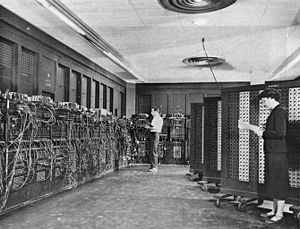
\includegraphics[width=.9\columnwidth]{300px-Eniac.jpg}
\end{center}
\caption{Photograph of Glen Beck (background) and Betty Snyder
  (foreground) programming the ENIAC in BRL building 328. (U.S. Army
  photo), downloaded from wikipedia. This photo was automatically
  resized to ${\frac{9}{10}}$ of the text column using
  the \textbf{includegraphics} command.}
\end{figure}

\section{ASIDE}
I copy/pasted the aside section fomr our recent vlhcc paper for reference. I have added some additional content to make it fit


In this section we describe our prototype interactive static analysis tool, named ASIDE. This version of ASIDE supports both interactive annotation and interactive static analysis. It is implemented in the form of an Eclipse plugin, and it runs inside the IDE. As developers type, static analysis is carried out behind the scenes. When issues are detected, developers are shown warnings similar to a colored icon on the left margin of the code editing window. These warnings are also accompanied by highlighted text. Developers can then click on these icons and view a contextualized description of why the warning is there (change wording later). Developers can then choose from a variety of quick fixes, as shown in figure (add this later). These quick fixes then auto generate code to solve the issue. One of these quickfixes, called "Read More" opens a webpage which contains much more contextualied help for the specific issue. For sql injection warnings, autogenerated code options were not provided, since prepared statements should be used to solve the problem. A screenshot showing a vulnerability warning produced from interactive static analysis is below:

screenshot showing red devil warning. 

Developers can choose one of these ``quickfixes'' as Eclipse refers to them by double clicking them. A single click reveals information about what the option will do if it is chosen. The screenshot below shows an example of the supporting information for the "Allow Only Letters and Numbers" option.

screenshot showing letters and numbers description

In many previous studies with static analysis tools, we found that developers wanted to see contextualized information about vulnerability warnings. To support this, we added this functionality to our current prototype. When information about a quick fix is displayed, it includes contextualized information about the actual code the developer is currently working on. In figure X (previous figure), notice how the description says "DESCRIPTION TEXT HERE". This refers to a function called "FUNCTION NAME HERE" that exists in the code the developer is working on.

All of the vulnerability warnings shown thus far have involved input validation issues. These are issues which can be fixed simply by validating the incoming input so that tainted data does not enter the program. However, the interactive static analysis portion of ASIDE's functionality also supports output encoding issues. These are issues in which cross site scripting or log poisening could occur due to untrusted output being printed to a sink, or area in which malicous code could execute. Output encoding issues were represented by the same icon, in the same location. However, the options were different. As with the input validation warnings, output encoding warnings display contextualized help when a quick fix is selected. The screenshot below shows an example vulnerability warning which can be resolved via output encoding.

screenshot showing output encoding.


In addition to the condensed contextualized help available when selecting a quick fix, more detailed contextualized help was also available. This was implemented in the form of a web page with detailed information that described the problem, why the tool felt something was wrong, and the suggested solution. Each web page was styled, and various tabs could be expanded and closed as needed. Each web page was accessible via a quick fix called ``Read More'' which was one of the available quick fixes. An example contextualized help ``Read More'' page is shown below.

read more screenshot here.



Aside also supports interactive anntation. The Interactive annotation portion of the tool takes as input: (a) Abstract Syntax Trees (ASTs) of the application generated by Eclipse JDT or PDT, and (b) a set of security sensitive operations such as operations that read or modify sensitive databases. ASIDE then uses these to generate requests within the IDE for the developer to annotate security related decisions, see Figure~\ref{fig:annotationRequest}. This request is indicated by a yellow highlight of the sensitive code, and a yellow question mark alongside the code. We chose a question mark to try and convey that the tool is requesting information, not indicating anything wrong with the code. Thus, in the example in Figure~\ref{fig:annotationRequest}, the developer was asked to indicate where access control checks are located for the function \textit{updateAccount} that accesses sensitive database tables. Clicking on the icon or code provides a menu where the developer can access ASIDE explanations, as well as choose to enter annotation mode. 

In annotation mode, the developer would then highlight the statements performing access control for the sensitive operation, highlighted in green in Figure~\ref{fig:completedRequest}. In doing so, the developer is reminded to add such checks, if they are not already implemented. ASIDE indicates the annotation with a green highlight and a small green diamond next to the code. The sensitive operation also turns green when an annotation is added, with the icon changing to a green check mark. Even when there are no vulnerabilities detected and no further interaction required by ASIDE, we choose to keep the green icons visible to allow developers to further modify annotations and interact with ASIDE as they continue development. Once the annotation is made, ASIDE leaves annotation mode and the developer returns to the task of coding. 

With the annotations provided by the developer, static analysis is used to detect vulnerabilities. This currently utilizes a path coverage algorithm, which analyzes all paths from the web entry point of the code to the security sensitive operation, ensuring that all paths go through the annotated security checks. Paths without all of the checks are flagged as potential vulnerabilities, and presented as warnings to the developer.  Alternatively, repeated sensitive operations are detected, such as other calls to the function \textit{updateAccount}, and differing access control logic is flagged as a potential vulnerability. In other words, our tool utilizes a standard static analysis technique that assumes that the same operations should be protected by the same access control logic. If the annotated access control logic differs between multiple instances of the same operation, all of those instances are flagged as containing a potential vulnerability. Due to space constraints, we cannot provide all the details of how our path coverage and vulnerability detection algorithm work, but it is fully explained in our recent publication \cite{sacmat2015}.  

A vulnerability warning would be presented as shown in Figure~\ref{fig:warning}, with the red highlighted code and red flag icon. Clicking on the warning would again provide a menu of options, brief explanations of the warning (e.g. the access control logic and the other operations that are related to this warning), and access to more detailed help regarding access control vulnerabilities. Developers can fix the warning by changing the code, and re-annotating the correct access control. Alternatively, they can dismiss the warning if they decide there is not a vulnerability.






\begin{figure}[h]
\centering
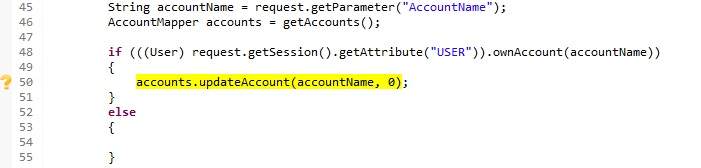
\includegraphics[width=0.5\textwidth]{annotationRequest}
\caption{Annotation request in Gold Rush, shown with a yellow highlight and question mark icon.}
\label{fig:annotationRequest}
\end{figure}

\begin{figure}[h]
\centering
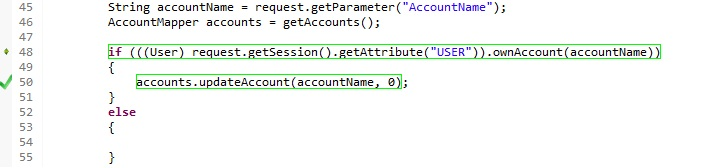
\includegraphics[width=0.5\textwidth]{completedRequest}
\caption{An annotation and annotation request that have been completed in Gold Rush. The completed request is shown with a green highlight and green checkmark icon.}
\label{fig:completedRequest}
\end{figure}

\begin{figure}
\centering
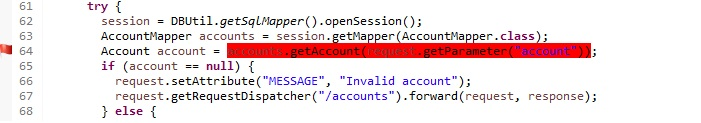
\includegraphics[width=0.5\textwidth]{warning}
\caption{ASIDE example with sample code in Gold Rush. A warning is displayed on line 64}
\label{fig:warning}
\end{figure}



\section{Methodology}
We designed a user study to examine user interaction with the contextualized version of our interactive static analysis and interactive annotation prototype. First, we wanted to assess how well our tool ``answered'' developer's questions from our previous study. Second we wanted to assess how intuitive our interface is for developers. Third, we wished to understand developer's perceptions of our combined prototype. Lastly, we wanted to assess the effectiveness of our tool in assisting developers with understanding potential security vulnerabilities regarding sql injection, cross site scripting, and access control.

We recruited actual professional developers from various companies to conduct our study. There job titles included the following: (list all job titles).  They had an average of X years of experience as professional Java Developers. To recruit these developers, we used a snowball sample. We asked developers we knew, and we asked them to recommend additional participants. To compensate developers for their time, we awarded a  \$25 gift card to each participant. A participant demographics table is shown below.

Participant demographics table here

Participants interacted with ASIDE running on a project called Gold Rush, an internally developed Java-based banking application (99 files) to teach web application security. When participants were interested, we would send them an email with a consent form. Participants would then individually book a time to perform the study and reply back saying they consent. At the booked time, they would call us from a remote location, and login to our computer through the use of remote desktop software. Participants were then given a brief introduction to ASIDE. They were then shown and allowed to interact with a trainer example, which consisted of one input validation warning. The purpose of the example was to answer any questions they had before beginning and to account for Eclipse interface quirks which could not be removed or fixed in our current prototype.

We would then show the participant a serious of warnings and ask participants which option they would choose. Afterwards, we would ask them a set of questions, which were the same for all of the warnings. If they did not visit the ``Read More'' pages, we would prompt them to do so when they had examined all of the warnings. Once they had observed all of the warnings, we showed them a very brief example of an annotation request and an annotation. During the demonstration, the researcher would perform an annotation. Then, the participant was asked to create annotations for two annotation requests. After each of these, we asked several questions. The questions were the same for each of the annotation requests. Once this was done, we asked several questions about aside as a whole and asked them to provide answers for a demographic survey. Throughout the study, participants were shown the same warnings and annotation requests, in the same order. Call recording and screen recording software were used to capture the activities of the participant on screen and the responses. The primary author performed open coding on the transcriptions and notes, to determine performance and look for common patterns and interesting responses.


\section{Results}


Preventing and understanding potential attacks
Is this a real vulnerability? (7)		Very commonly, developers would check to see whether or not a vulnerability was exploitable to determine whether or not it was real. In 21 instances, 8 developers explicitly or implicitly indicated that whether or not code was vulnerable depended on whether or not a perceived exploit was possible. If no exploit was observed or the developer determined that an exploit was not possible, the code was considered to not be vulnerable. This led to some developers pronouncing some vulnerability warnings as false positives, since they did not appear exploitable. 

“it might not be the most effective cross-site scripting but in this case I feel like just because of the way current users initialize, it's not really that big of an issue” -p13

“If it's not sanitized it's known as a XSS attack….It's going to depend on the implementation of account.”-p1


This phenomenon was particualry noticable in the case of output encoding warnings. In these cases, unsantized output was printed to a sink, such as a webpage. X developers indicated that this was not a vulnerability since the code should originate from a trusted source. In these cases, all of the developers explicitely stated that input validation should be performed where data originates, and once in the system it should be considered trusted. However, if an attacker was able to bypass this, or if input validation was not performed at a taint source, the code would then be exploitable in a cross site scripting or log poisoning attack. Since this code did not appear exploitable, these developers did not consider the code to be vulnerable. In X cases, this caused them to take no action and pronounce the warning to be a false positive. 

“I would think that we would take care of this somewhere else, I would think we wouldn’t want any kind of injected, we would validate the user name at the time when they select it not here” -p3


often developers would look to see if it was exploitable to determine if it was real. Developers also evaluated whether or not the vulnerability warning was a false postive. 
What are the possible attacks that could occur? (5)	The developers would generally believe the tool, rather than ask the question. Developers only discussed the vulnerability from the perspective of the attacker in 3 instances. This is surprising, as it suggests that developers have not been taught to do this when assessing whether or not code is vulnerable. However, developers would almost always trace the code, thinking about where malicious content may enter, and how that would effect the line that aside flagged.

“the issue here is that they would put some code in the username and they would evaluate that”-p3

Why is this a vulnerability? (3)	Common in cases of planted false positives, also on output encoding. Participants often questioned why a line was vulnerable. It is important to point out that they often did not question why the tool suggested that the line was vulnerable. However, they would frequently think about the path of execution and use it to make a determination on whether or not aside had produced a false positive or the warning was legitimate. This was particulary noticable during annotation request tasks.

How can I prevent this attack? (3) Generally developers would use aside quick fixes to resolve vulnerability warnings. However, two developers explicitly mentioned that they would write their own validators with regular expressions rather than use Aside's quick fix. This aligns with our previous studies in which knowledgeable developers chose to implement their own fixes if they understood the problem and the solution. In these cases, both developers expressed very high confidence that their solution would fix the vulnerability. In cases where developers chose aside quick fixes, they were very hesitant to commit to saying that the chosen solution would make the code secure without viewing and testing the generated code.  After choosing a quick fix for each vulnerability warning, developers were asked to respond with a number from 1 to 10 (with 1 being very weak and 10 being very strong) indicating how confident they were that the chosen quick fix would fix the problem. Among all tasks and all developers, the average given was Y.  In X cases, developers asked if they should respond with an assumption that the generated code worked.  After the researcher told them “yes,” they responded with an average of Z for those warnings. This data suggests that developer confidence of vulnerability resolution depends on two things:

1. Confidence that the generated code will work properly for it's intended problem

2. Confidence that the correct quick fix was chosen for the current problem

Based on the responses from the developers who asked if they should assume the generated code worked, it appears that developers were more hesitant to trust the robustness of the generated code than the applicability of their quick fix selection. This suggests that tools which provide quick fixes for vulnerabilities should generate code which is well commented and easy to read and understand in order to gain the developers' trust. Effort should also be put into convincing the developers of the effectiveness of the solution. 

It is also important to point out that developers also expressed concern over a quick fix when it did not perfectly fit the data. For example, ASIDE provides a quick fix called “Allow Only Letters and Numbers.” In cases where the incoming data should only be a number or a letter, developers were very hesitant to trust the applicability of the solution. However, since it is impossible to cover every possible use case, it is recommended that tools provide fixes for data types instead of use cases. For example, “Allow Only Numbers” is likely a better option than “Allow Only Social Security Numbers.” This approach would allow the tool to handle validation for security, while allowing the developer to fine tune the output for a custom application.



 When asked to provide a number from 1 to 10 incating how confident they were that their chosen solution would fix the problem, they would ask if they should answer the question without viewing the  provided an average Perhaps this stemmed from a lack of security training, or a possible subconscious feeling that they could be held responsible if they claimed it was secure and it was later found to be vulnerable. 
How can I replicate an attack to exploit this vulnerability? (2)	Most of our developers (n =11)  did not think from the perspective of the hacker and did not consider black box testing, white box testing, or any form of penetration testing. However, they would often trace the code and consider the effects of certain inputs.
What is the problem (potential attack)? (2)		Sometimes, developers were more concerned about logic flaws and application semantics in cases of cross site scripting than the actual vulnerabilities themselves. In other words, if an application allowed a balance to be changed through a url parameter, even if the application was designed to work in this way, it was percieved to be a much higher risk issue than the actual cross site scripting issue that aside flagged.  Perahps this stems from a primary job task of ensuring that implemented requriements match actual program requirements. 


Understanding Alt Fixes and Approaches
Does the alternative function the same as what I’m currently us-
ing? (6) Many developers had concerns about trusting the tool's solutions to the problems and would want to write their own validation functions
What are the alternatives for fixing this? (4) same as above
Are there other considerations to make when using the alterna-
tive(s)? (3) Participants would often scan the code when thinking about alternative solutions to the problem to make sure that it agreed with the logic
How does my code compare to the alternative code in the example
I found? (2) n/a not their code
Why should I use this alternative method/approach to fix the vul-
nerability? (2) Participants would often try to justify why they would not trust the tool and would instead use their own technique by talking about how it would be more specific to the use case.
Does the alternative function the same as what I’m currently us-
ing? (6) Participants did consider whether or their fix was the same but placed a higher “trust” in their own.
What are the alternatives for fixing this? (4) Participants considered alternative solutions, particulary when the santization was too broad.
Are there other considerations to make when using the alterna-
tive(s)? (3) n/a
How does my code compare to the alternative code in the example
I found? (2) n/a not their code
Why should I use this alternative method/approach to fix the vul-
nerability? (2) Participants justified why they would use their own approach.


 Assessing the Application of the Fix

Will the notification go away when I apply this fix? (5) Participants sometimes questioned whether or not the vulnerability warning would disappear when a fix was applied. However, they questioned this much less than expected from the prior study. This could have partly been the case because they were not actually choosing quickfixes and were instead telling us which one they would choose. However, due to the results of the previous study, it is recommended that tools keep some sort of overview of resolved issues, so that developers can access them again if necessary.
How do I use this fix in my code? (4) Participants did not often question how to use a fix, perhaps this is because aside provided auto generated quick fixes that do not require further work. This may povide a significant boost to the effectiveness of static analysis since it reduces or removes the possiblity of the developer improprely implementing a fix.
How do I fix this vulnerability? (4) Developers did question how to fix vulnerabilities. There was much cofusion over santize html and santize url. Some wanted to choose both. Most chose correctly, but expressed doubts that perhaps the other option was correct.  Developers also wanted a quick fix for everything, many (most) of them actually suggested ways of programmaticaly generating prepared statements to enable quick fixes for sql injection.
How hard is it to apply a fix to this code? (3) Participants did not question the difficulty of applying a quick fix. This may be partly due to the fact that it was a simple double click option that auto generates code. This again helps deal with errors which may result from developers incorrectly applying fixes. 
Is there a quick fix for automatically applying a fix? (2) Developers desired quick fixes whereever possible. In most cases, they did not quesiton whether or not a quick fix was provided since it was provided to them by the aside tool for issues in which output encoding or input validation was necessary.
Will the code work the same after I apply the fix? (2) Some participants expressed concern that the quick fix could break the code, but most trusted it not to alter the functionlity. However, they wanted the sanitization to be very specific to the type of characters which were valid in the given context.
What other changes do I need to make to apply this fix? (2) Participants would often comment if they save some sort of logic issue or functionaltiy concern in addition to the vulnerability. In many cases, they expressed concern that more steps may be necessary to properly secure the code.

 Relationship Between Vulnerabilities (4){3}

Are all the vulnerabilities related in my code? (3) Developers did not usually question whether one vulnerability was related to another. This could be partly because they were told to focus on one at a time. However, in cases where the semantics of the application did not make since (eg. Adding money to account via http parameter), they would often discuss this as being a more serious issue than the vulnerability itself 
Does this other piece code have the same vulnerability as the code I’m working with? (1)? Many participants noticed when the  input validation warning was repeated and called attention to it. However, most of them also correctly identified it as a false positives

Locating Information

Where is this used in the code? (10) Incredibly common. Developers moved far slower than students making annotation in the previous study. They almost always evaluated the code heavily before deciding what action to take. In most cases, whether or not they considered the code to be vulnerable depended on where it was used in the code and its purpose, rather than the fact that it was unvalidated input or unencoded output
Where are other similar pieces of code? (4) Developers often browsed the code heavily. Although they did not explore other files, in many cases they verbally expressed interest in knowing the purpose of other pieces of code. In many cases, they made security decisions based on assumptions about what this code did or did not do. 
Where is this method defined? (1) Developers did not seek out other files to find where methods were defined. However, they verbally expressed interest. They may have done this if the study did not focus on one file at a time.

Control Flow and Call Information

Where is the method being called? (10) (Also incredibly common. Developers frequently wanted to know the context of the code before making any security decisions. They did not seem to operate on the notion that “unvalidated data is bad, sanitize all” instead, they only considered it necessary if it actually ended up in some sensitive sink.
How can I get calling information? (7) Developers often wandered how the tool provided the results that it did. Many of them expressed a desire to know the basics behind how the tool was able to provide the warnings and annotation requests. In previous studies, they wanted to know WHY the tool thought the line was vulnerable. In this study, the contextual help seemed to answer the why question, but not th e how question.
Who can call this? (5) Participants considered the context to be very important in determining a solution.
Are all calls coming from the same class? (3) n/a same as above
What gets called when this method gets called? (2) Participants often expressed uncertainty about whether or not a fix was correct. In some cases, they mentioned explicitely that it was due to not fully understanding the underlying code.

Code Background and Functionality

What does this code do? (9) Participants felt it necessary to understand the application's functionality before applying a fix. Most of the time spent thinking was spent trying to understand the underlying code. Participants often talked about how the code worked and justified their option choice based on it.
Why was this code written this way? (5) Partipipants would sometimes critique the code, particulary when they identified an issue in which the application logic did not make sense in a real world application.
Why is this code needed? (3) Participants sometimes expressed confusion over uneeded code and questioned whether or not it contributed to the vulnerability
Who wrote this code? (2) Participanrts often evaluated the messages based on whether it was to be viewed by a junior developer or an experienced developer. Some also expressed concern about the training of other developers when viewing code which was vulnerable, particulary with sql injection.
Is this library code? (2) n/a
How much effort was put into this code? (1) Participants were informed that this was an example banking application and was not a real bank. 

Application Context and Usage

What is the context of this vulnerability/code? (4) The context of the vulnerability was very important. If a vulnerability did not appear exploitable, most participants did not consider it be a vulnerability
Is this code used to test the program/functionality? (4) Participants did not question whether or not certain methods were part of debugging code. However, this application was far simpler and more compact than iTrust.
What is the method/variable used for in the program? (3) Participants did ask what certain methods and variables were used for, especially if it seemed relevant to the warning or annotation request.
Will usage of this method change? (2) Participants did not seem concerned about whether or not the context of when certain methods are called would actually change. It is possible, based on other findings detailed above, that they would dismiss an issue as not a vulnerability due to not being exploitable, only to have the application context change and an exploit appear later.
Is the method/variable ever being used? (2) They did question whether or not certain methods are variables were actually used. Many became suspicious of vulnerabilites when suspicious methods or variables were found to be unused. This may be because the code was perceived to be “bad” and “bad” code may be more likely to contain vulnerabilities.

End user Interaction

Is there input coming from the user? (4) Participants frequently questioned the source of the data. If data came from some “trusted” source, such as the session or the database,  many assumed that it was to be trusted and did not need to be encoded, even if how it arrived at this trusted source was unknown. However, many of these participants did emphasize a need for input validation if the data came from untrusted sources.
Does the user have access to this code? (4) This was a common issue. One developer compared the permissions of the file to the linux filesystem, stating that users already had read permission, and questioned whether they should have read permission, or read and write permission. It is interesting that participants would think about permissions in this context, rather than based on sensitive operations and logic checks.
Does user input get validated/sanitized? (4) This was also common. Many developers wanted to know if the data was already santized. They did not see a need for dupliate santization, even though the comuting resource cost of the sanitization is very low.

Individuals

Do I understand? (3) Participants did sometimes question themselves and dropped many indicators of a low confidence answer. Often, they avoided direct answers to whether or not something was exploitable or vulnerable, or whether or not the chosen fix would work. Perhaps they were cautios due to the vast amount of exploits available when certain vulnerabilites are present. 
What should I do first? (2) n/a
What was that again? (2) Participants did often reread the code to try to gain an understand of the purpose of the code and what the code was actually doing.
Is this worth my time? (2) Most participants did not simply believe in a “click it, make the tool happy” approach, instead preferring to determine whether or not a certain issue needed to be solved or could be  safely dismissed.
Why do I care? (2) Most participants were very concerned about sql injection. However, they were not nearly as concerned or aware of cross site scripting, as indicated explicitely and in low confidence answers. In cases of cross site scripting, they perceived the issue to be less severe. They often asked many questions about the purpose of the annotation. Many did not fully understand the reason for creating annotations. They were not told about access control vulnerabilities, and it is possible that many did not understand what they were. It is also possible that they did not understand how the tool could detect mismatched annotations and detect vulenrabilies. They saw annotation more as a task they had to do for the tool, rather than providing input to the tool to help it detect issues. The phrase 
“ignorance is bliss” seems to come to mind.
Have I seen this before? (1) Partiipcants often reacted very quickly to cases they had personal experience with, paticulary sql injection. In cases where a warnign was repeated, such as the input validation warning, participants would often reason about the solution in the same way as they did the initial warning. They also would jusity any different solution based on the solution to the original warning
Where am I in the code? (1) Participants did browse the code and question their location, but more commonly the quesitons invovled the functioanlity of the code.

Concepts

What is this concept? (6) Partiicpants seldom questioned the concepts when using the tool, perhaps as a direct result of the contextualized help. Often they would get confused regarding prepared statements, since the tool did not provide a quick fix. However, they reacted very postiively to the additional help page and particularly appreciated the concrete examples.
How does this concept work? (4) Most partiicpants did read the descriptions, mostly for the heading, when clicking on issues. Most also felt that it explained the concept behind why a line was vulnerable. 
What is the term for this concept? (2) Most paticipants did not question the terminology since the tool provided it in the contextualized help.

Problem Solving/ Support

Can my team members/resources provide me with more informa-
tion? (5) Participants did qustion whether or not the tool was meant to be used standalone or as part of a project. They expressed desire for it to be done at the project level. However, some of them also expressed concern about embarrassment from others seeing their mistakes in code
Where can I get more information? (5) Partiipcants loved the contexutalized help pages, but many of them were not aware of how to actually find the contexualized help pages. When asked, many of them said that there first instinct would be to google the issue and read about it. They also expected the documentation to be less contextualized than it actually was. They often stated the need to double click and the appearance of read more as a quick fix were the reasons for not exploring it previously. 
What information is in the documentation? (5) Partiipcnats often read over the contextualized help in detail when the arrived at it. They loved the ability to expand and shorten sections as needed. They also loved copy/pastable concrete code examples. Perhaps this is due to the influence of stack overflow?
How do resources prevent or resolve this? (5) Participants did not often question how a technique from the contextualized help would prevent or resolve the problem. The contextualized help pages were able to convince the participants of the correct solution in all cases. Perhaps, because it was contextualized, it was perceived as “smart” and more likely to be correct. 
Is this a reliable/trusted resource? (3) Developers did not question whether the resource could be trusted. However, they did question the warnings and annotation requests themselves
What type of information does this resource link me to? (2) Participants who did not explore for more information often did this because they felt the information was likely to be inferior to what they would find on google. Somehow communicating that it is contexutalized may help to increase the odds of developers exploring the contextualized help


Unserstanding and Interacting with tools

Why is the tool complaining? (3) Participants often questioed how the tool was able to determine that a certain issue was going on, but did not usually question why the issue was flagged by the tool. This may have been due to the contexutalized help.
Can I verify the information the tool provides? (3) Participants expressed low trust in the quick fixes. When asked how confident they were that the solution they chose was correct, many of them expressed doubts, wishing they could see the code before deciding. Many of them said that they would choose a quick fix, and then evaluate it to determine whether or not it was correct.
What is the tool’s confidence? (2) Participants did not question the tool's confidence level. However, they were somehwat accurate at spotting false positives, less so in the case of annotation.
What is the tool output telling me? (1) Participants did question what the tool was trying to tell them in some cases, particularly in the case of cross site scripting and for annotation requests.
What tool do I need for this? (1) n/a
How can I annotate that these strings have been escaped and the
tool should ignore the warning? (1) Participants expressed desire to dismiss warnings and annotation requests which were false positives. They did not explicitely mention an annotaiton aprroach to do this.  Rather, they requested a quickfix. We have seen this in prior studies.

Vulnerability Severity and Raking

How serious is this vulnerability? (2) Unlike the previous participants, developers did not seem to share the same mental model of “scales” of vulnerabilties. They would often make a determineation of whether something was vulnerable or not vulnerable. They often would not say that somehting was “more vulnerable” or “less vulnerable” than other vulnerabilies. Perhaps this is due to greater training and security knowledge. However, they did question how severe the exploits of those vulnerabilties could be. In cases where the perceived explotis were minor, the vulnerability was considered less severe. SQL injection was seen as particulary severe. Cross site scripting resulting from tainted data in the system was seen as particulary not severe.
How do the rankings compare? (2) Participants did not compare severity rankings. Some research has shown that it may be best for tools to stop ranking vulnerabilties in terms of severity.
What do the vulnerability rankings mean? (2) n/a aside does not rank vulnerabilities
Are all these vulnerabilities the same severity? (1) Participants evaluated vulnerabilities on a case by case basis. They did not explicitely question whether or not vulnerabilities were flagged as the same severity level or a different severity level. Perhaps this was due to the way the interface communicates the issue. However, annotation requests were perceived as less severe than the warnings. 

Notification Text

What does the notification text say? (5) Participants did often reread the text from the aside warnings to try to fully determine what was meant by the wording. They sometimes suggested a standard template response with one section that explains why the line was flagged and other for explaining the consequences if the issue is left alone.
What is the relationship between the notification text and the code?
(2) Participants did question whether or not the text was a false positive. This meant they were evaluating the relationship between the text and the code. If it did not make sense, it helped them in determining whether or not it was a false postiive. They did examine the contextualized part of the messages thoroughly and more slowly than the rest of the message, which was static text. Perhaps they were looking to see if it made sense with the current code.
What code caused this notification to appear (2) As detailed previously, participants did question how the tool was able to generate warngins and annotation requests, particulary annotation requests. However, they did not percieve this to be as important as WHY a warning or request was shown.















Old notes here

On the whole, participants seemed to prefer the way ASIDE presented vulnerabilities to the annotation requests. Reason, similar to other tools? Harder? Presented at the end? No access control vulnerability explanation? Emphasis on these types of issues?. Some of them seemed to not understand the reasoning behind the annotations. Perhaps more training (like the last study) is needed. They also were not familar with the code, like the studetns in the previous study were.

Participants wanted quick fixes for everything. They suggested at ways to do it for sql injection and expressed a desire to have it for access control issues.

In terms of the quick fix options, participants hinted at a trade-off between specificity and generality. Particpants did not like "letters and numbers" for cases when only letters or only numbers was ideal. They wanted specific options that fit the specific issue.
 
While addressing the vulnerabilities, some participants griped that ASIDE didn't provide enough background information. Most of them did not attempt to open the contextualized help pages. However, when they found it or were shown it, they were almost always very very pleased to see it. Many suggested that they did not see it because it looked like another quick fix. Also, they didn't realize double clicking it would open a web page. They suggested a link in the descriptions of the other fixes would be better.

Participants were very good at choosing the right options for quick fixes. They moved a lot slower than the students from the previous annotation study, perhaps trying to be more careful. When they understood the annotation approach, they liked it, were skilled at it, and rated it well. Overall, particpants gave very favorable evaluations for the tool. Many likert scale questions were used and we expect those numbers to be favorable.
 
 

\section{Conclusions}
This paragraph will end the body of this sample document.
Remember that you might still have Acknowledgments or
Appendices; brief samples of these
follow.  There is still the Bibliography to deal with; and
we will make a disclaimer about that here: with the exception
of the reference to the \LaTeX\ book, the citations in
this paper are to articles which have nothing to
do with the present subject and are used as
examples only.
%\end{document}  % This is where a 'short' article might terminate

%ACKNOWLEDGMENTS are optional
\section{Acknowledgments}
This section is optional; it is a location for you
to acknowledge grants, funding, editing assistance and
what have you.  In the present case, for example, the
authors would like to thank Gerald Murray of ACM for
his help in codifying this \textit{Author's Guide}
and the \textbf{.cls} and \textbf{.tex} files that it describes.

%
% The following two commands are all you need in the
% initial runs of your .tex file to
% produce the bibliography for the citations in your paper.
\bibliographystyle{abbrv}
\bibliography{sigproc}  % sigproc.bib is the name of the Bibliography in this case
% You must have a proper ".bib" file
%  and remember to run:
% latex bibtex latex latex
% to resolve all references
%
% ACM needs 'a single self-contained file'!
%
%APPENDICES are optional
%\balancecolumns
\appendix
%Appendix A
\section{Headings in Appendices}
The rules about hierarchical headings discussed above for
the body of the article are different in the appendices.
In the \textbf{appendix} environment, the command
\textbf{section} is used to
indicate the start of each Appendix, with alphabetic order
designation (i.e., the first is A, the second B, etc.) and
a title (if you include one).  So, if you need
hierarchical structure
\textit{within} an Appendix, start with \textbf{subsection} as the
highest level. Here is an outline of the body of this
document in Appendix-appropriate form:
\subsection{Introduction}
\subsection{The Body of the Paper}
\subsubsection{Type Changes and  Special Characters}
\subsubsection{Math Equations}
\paragraph{Inline (In-text) Equations}
\paragraph{Display Equations}
\subsubsection{Citations}
\subsubsection{Tables}
\subsubsection{Figures}
\subsubsection{Theorem-like Constructs}
\subsubsection*{A Caveat for the \TeX\ Expert}
\subsection{Conclusions}
\subsection{Acknowledgments}
\subsection{Additional Authors}
This section is inserted by \LaTeX; you do not insert it.
You just add the names and information in the
\texttt{{\char'134}additionalauthors} command at the start
of the document.
\subsection{References}
Generated by bibtex from your .bib file. Run latex,
then bibtex, then latex twice (to resolve references)
to create the .bbl file. Insert that .bbl file into
the .tex source file and comment out
the command \texttt{{\char'134}thebibliography}.
% This next section command marks the start of
% Appendix B, and does not continue the present hierarchy
\section{More Help for the Hardy}
The sig-alternate.cls file itself is chock-full of succinct
and helpful comments. If you consider yourself a moderately
experienced to expert user of \LaTeX, you may find reading
it useful but please remember not to change it.
%\balancecolumns % GM June 2007
% That's all folks!
\end{document}
